\chapter{系统设计}
\label{chap:systemDesign} 

系统设计,讲讲怎么设计的吧。

\section{xx架构设计}

xx架构设计

游戏设计详细流程如图\ref{fig:gameFrame}所示。

\begin{figure}[H]
  \centering
  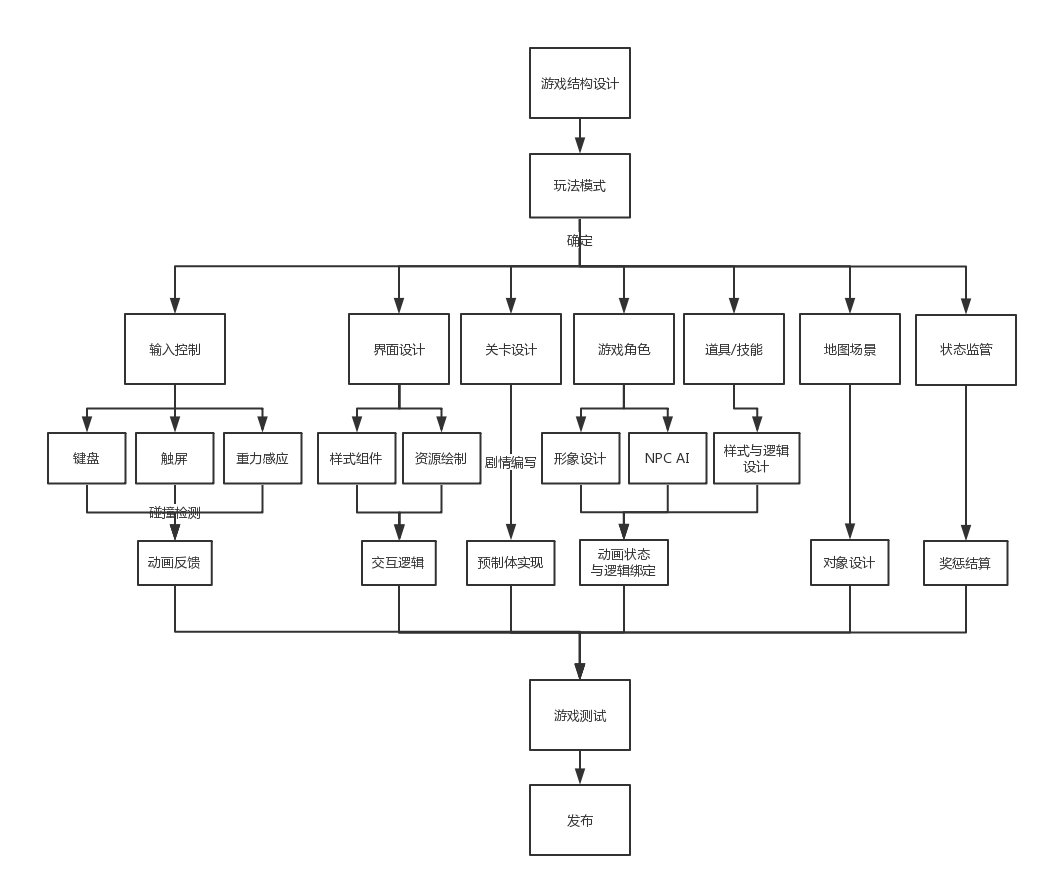
\includegraphics[width=15cm]{gameFrame}
  \caption{游戏结构设计}
  \label{fig:gameFrame}
\end{figure}

\subsection{项目结构}
\label{sec:folderStructure}

描述一下

游戏程序目录结构划分如表\ref{tab:gameRoot}所示。

这里是三线表的用法

\begin{table}[htb]
  \centering
  \begin{minipage}[t]{0.8\linewidth} % 如果想在表格中使用脚注,minipage是个不错的办法
  \caption[游戏主程序目录]{游戏主程序目录}
  \label{tab:gameRoot}
    \begin{tabularx}{\linewidth}{lX}
      \toprule[1.5pt]
      {\heiti 文件/文件夹名} & {\heiti 描述} \\\midrule[1pt]
      .git & git 版本管理目录 \\
      .vscode & VS Code 编辑器工作区配置文件目录 \\
      assets & 资源分类目录,放置游戏中所有本地资源、脚本和第三方库文件 \\
      build & 打包构建目录,存放目标平台的构建工程 \\
      docs & 游戏策划目录 \\
      library & library 是将 assets 中的资源导入后生成的,在这里文件的结构和资源的格式将被处理成最终游戏发布时需要的形式\cite{cccManual} \\
      local & 包含该项目的本地设置,包括编辑器面板布局,窗口大小,位置等信息 \\
      node\_modules & npm 扩展包存储目录 \\
      settings & 保存项目相关的设置 \\
      temp & 临时文件存储目录 \\
      .gitattributes & 游戏中使用到了许多图片资源,有些资源采用 Photoshop 自行绘制,故会产生 psd 文件,所占位置较大,采用了 Git LFS 进行管理 \\
      .gitignore & Git 版本控制过滤规则文件 \\
      creator.d.ts & Cocos Creator 语法提示文件 \\
      package.json & npm 包信息文件 \\
      project.json & 记载当前使用的引擎类型和插件存储位置 \\
      README.md & 本游戏程序说明文件 \\
      \bottomrule[1.5pt]
    \end{tabularx}
  \end{minipage}
\end{table}

\subsection{碰撞管理与物理系统设计}

可见的物体均模拟物理环境下的碰撞,存在不同的碰撞分组。
不同分组之前进行碰撞时,根据分组设定,触发不同的回调函数。

分组管理如表\ref{tab:group}所示。

多行多列的表格

\begin{table}[htbp]
  \centering
  \caption{分组管理}
  \label{tab:group}
  \begin{minipage}[t]{0.8\textwidth} 
    \begin{tabularx}{\linewidth}{|l|X|X|X|X|X|X|}
      \hline
      \textbf{分组名} & {gravity} & {scene} & {bullet}  & {enemy} & {player} & {default} \\ \hline
      {default} & & & & & & \\ \hline
      {player} & √ & √ & √ & √ & √ & \\ \hline
      {enemy} & & √ & √ & √ & √ & \\ \hline
      {bullet} & √ & √ & √ & √ & √ & \\ \hline
      {scene} & & √ & √ & √ & √ & \\ \hline
      {gravity} & & & √ & & √ & \\ \hline
    \end{tabularx}\\[2pt]
  \end{minipage}
\end{table}

xxx

\begin{table}[htbp] 
  \centering
    \caption{\label{tab:rigid}刚体属性} 
    \begin{tabular}{lcl} 
      \toprule[1.5pt]
      {\heiti 属性} & {\heiti 类型} & {\heiti 描述} \\\midrule[1pt]
      % \midrule 
      linearDamping & Number & 线性速度衰减系数 \\
      angularDamping & Number & 角速度衰减系数 \\
      linearVelocity & Vec & 线性速度 \\
      angularVelocity & Number & 角速度 \\
      density & Number & 密度 \\
      friction & Number & 摩擦系数 \\
      restitution & Number & 弹性系数 \\
    \bottomrule[1.5pt]
    \end{tabular} 
\end{table}